おそらくあなたはMVCのデザインパターンについて聞いたことがあると思います。Modelはデータを処理を、Viewは表示結果を、Controllerはユーザのリクエストの制御を行います。Viewレイヤーの処理では、多くの動的な言語ではどれも静的なHTMLの中に動的言語が生成したデータを挿入します。例えばJSPでは\texttt{<\%=....=\%>}を挿入することで、PHPでは\texttt{<?php.....?>}を挿入することで実現します。

下の図でテンプレートのメカニズムについてご紹介します

\begin{figure}[H]
  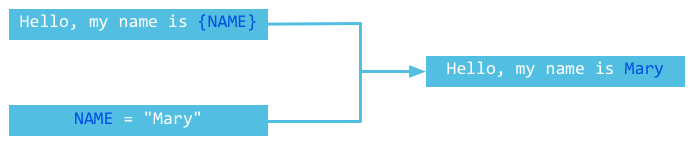
\includegraphics[width=14cm]{7.4.template.png}
   \label{図7.1}
   \caption{テンプレートのメカニズム図}
\end{figure}


Webアプリケーションがクライアントに返すフィードバックの情報の中の大部分の内容は静的で不変です。また少ない部分でユーザのリクエストによって動的に生成されるものがあります。例えばユーザのアクセスログリストを表示したい場合、ユーザ間ではログデータが異なるのみで、リストのスタイルは固定です。この時テンプレートを用いることで多くの静的なコードを使いまわすことができます。
